% Praktischer Teil
\section{Results}
\label{sec: results}

\subsection{Included Weather Stations}

From the 3D-Paws project (see \autoref{sec: 3d_printed_stations}), measurements from three different weather stations in recent years were obtained. The stations are located in Marshall, Colorado; Vienna, Austria; and Barbados, Caribbean.

% 3 images side by side with available weather stations
\begin{figure}
\centering
\begin{subfigure}{0.672\textwidth}
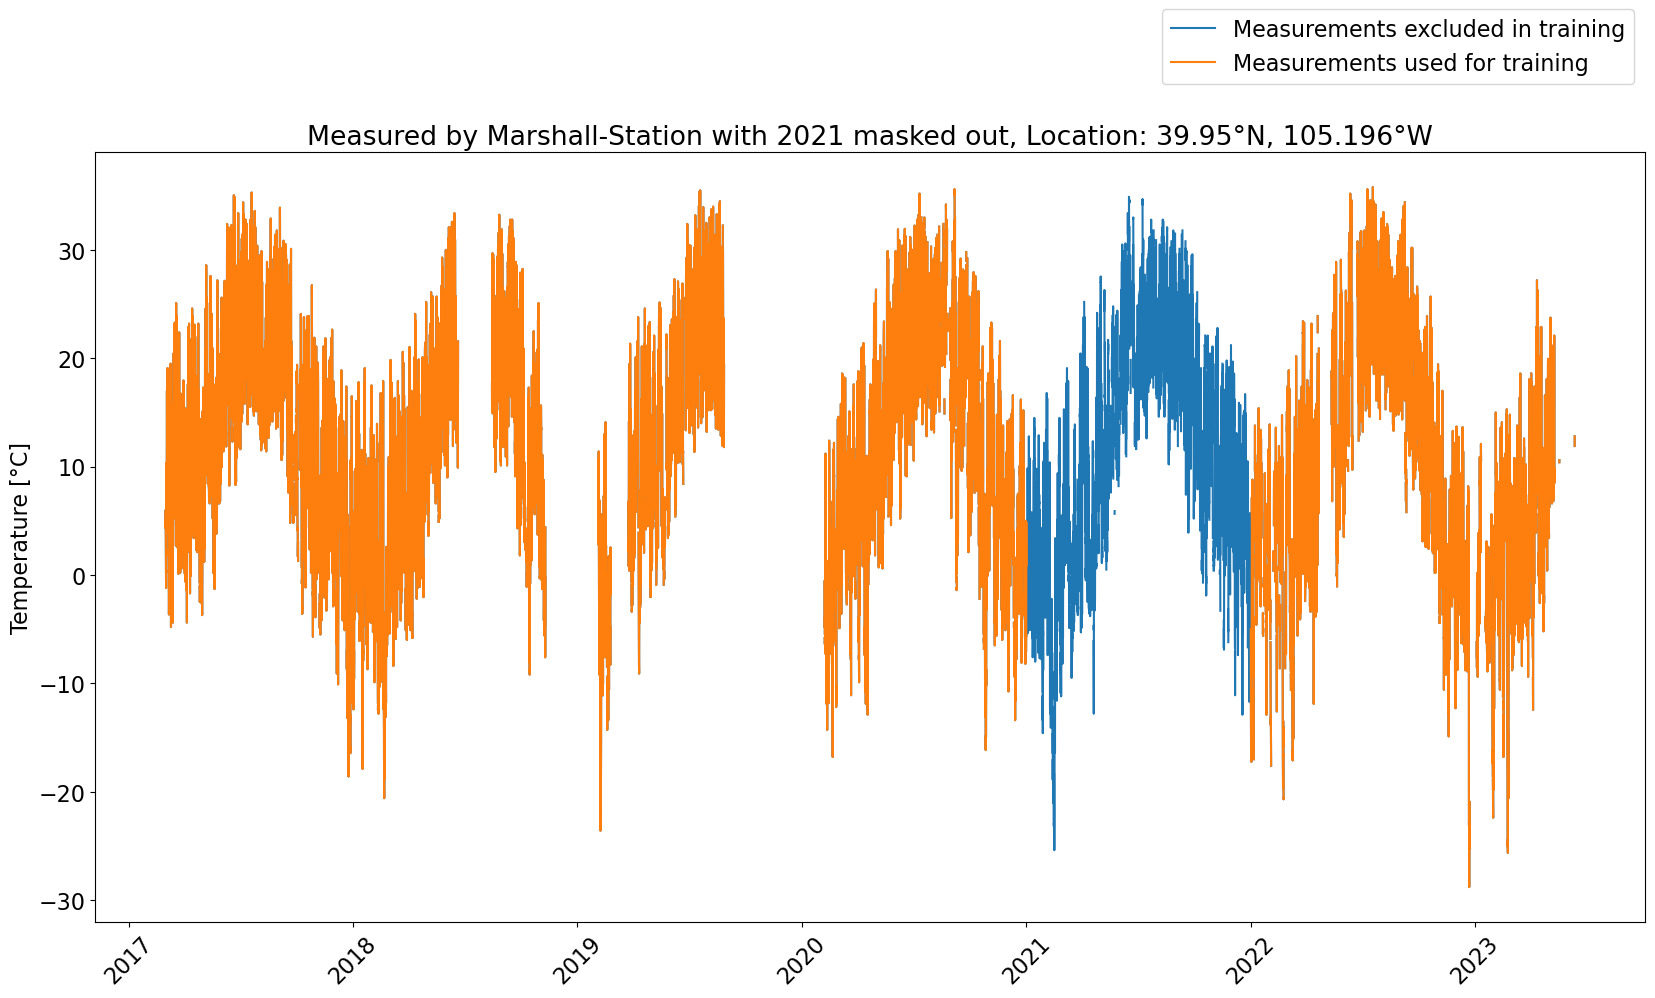
\includegraphics[width=\textwidth]{resources/images/charts/marshall_available_measurements.png}
\caption{Station in Marshall, Colorado, USA}
\label{fig: available_measurements_marshall}
\end{subfigure}
\begin{subfigure}{0.672\textwidth}
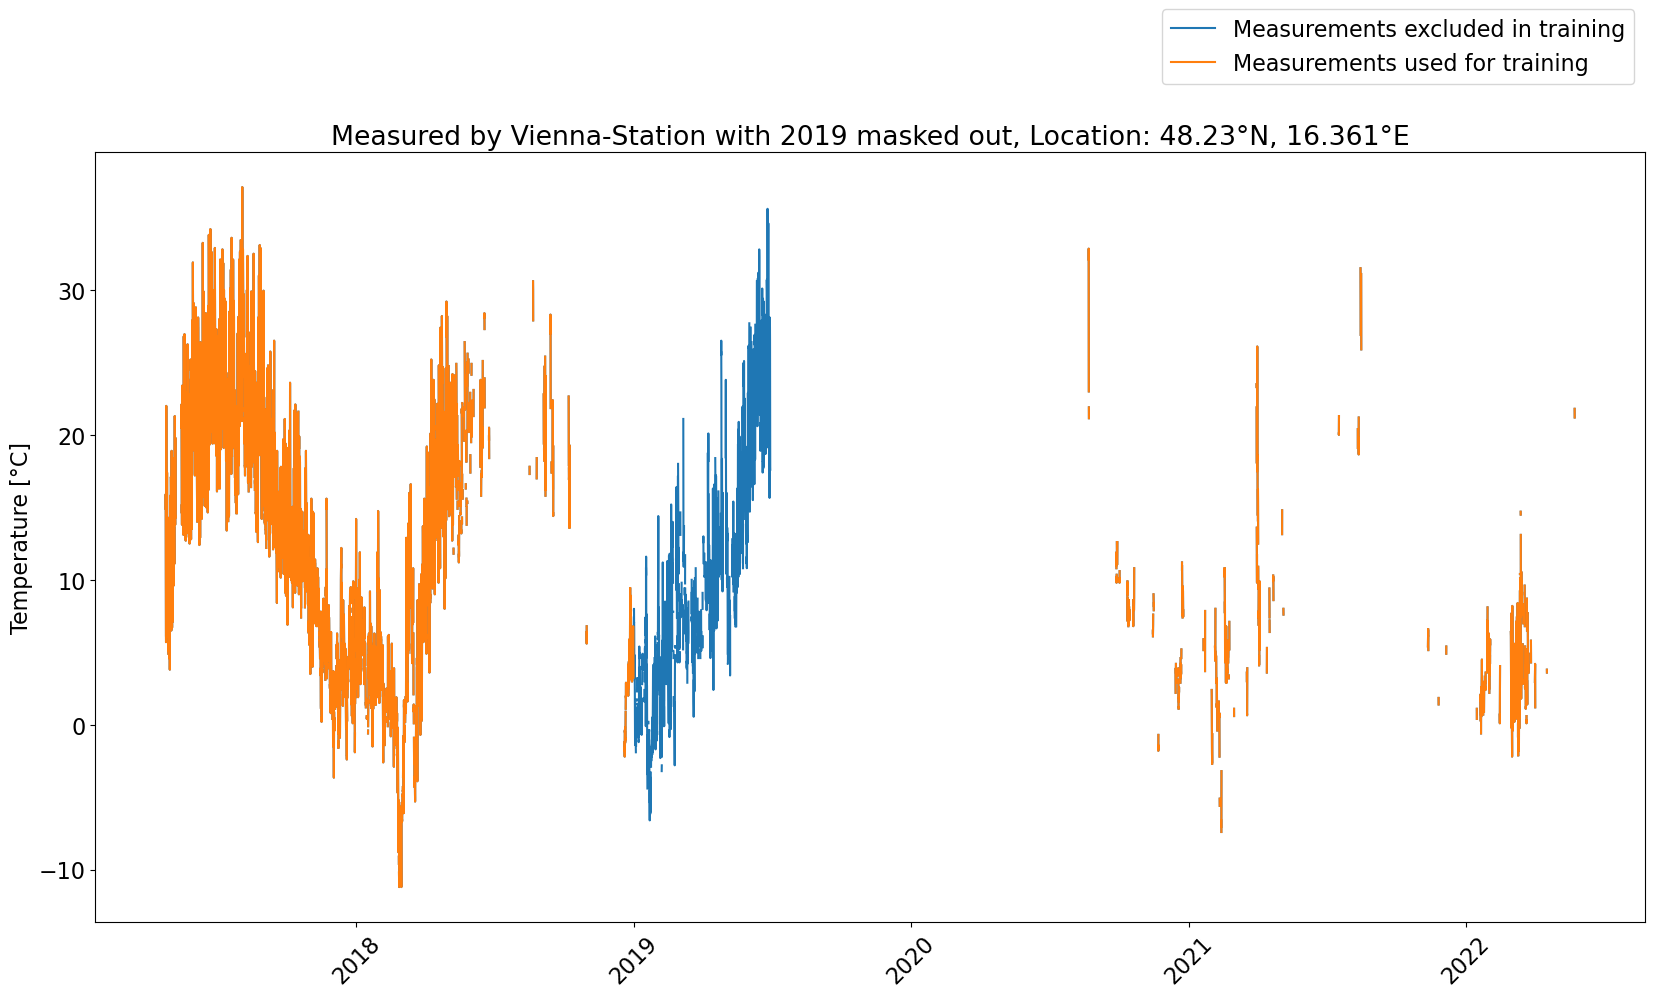
\includegraphics[width=\textwidth]{resources/images/charts/vienna_available_measurements.png}
\caption{Station in Vienna, Austria}
\label{fig: available_measurements_vienna}
\end{subfigure}
\begin{subfigure}{0.672\textwidth}
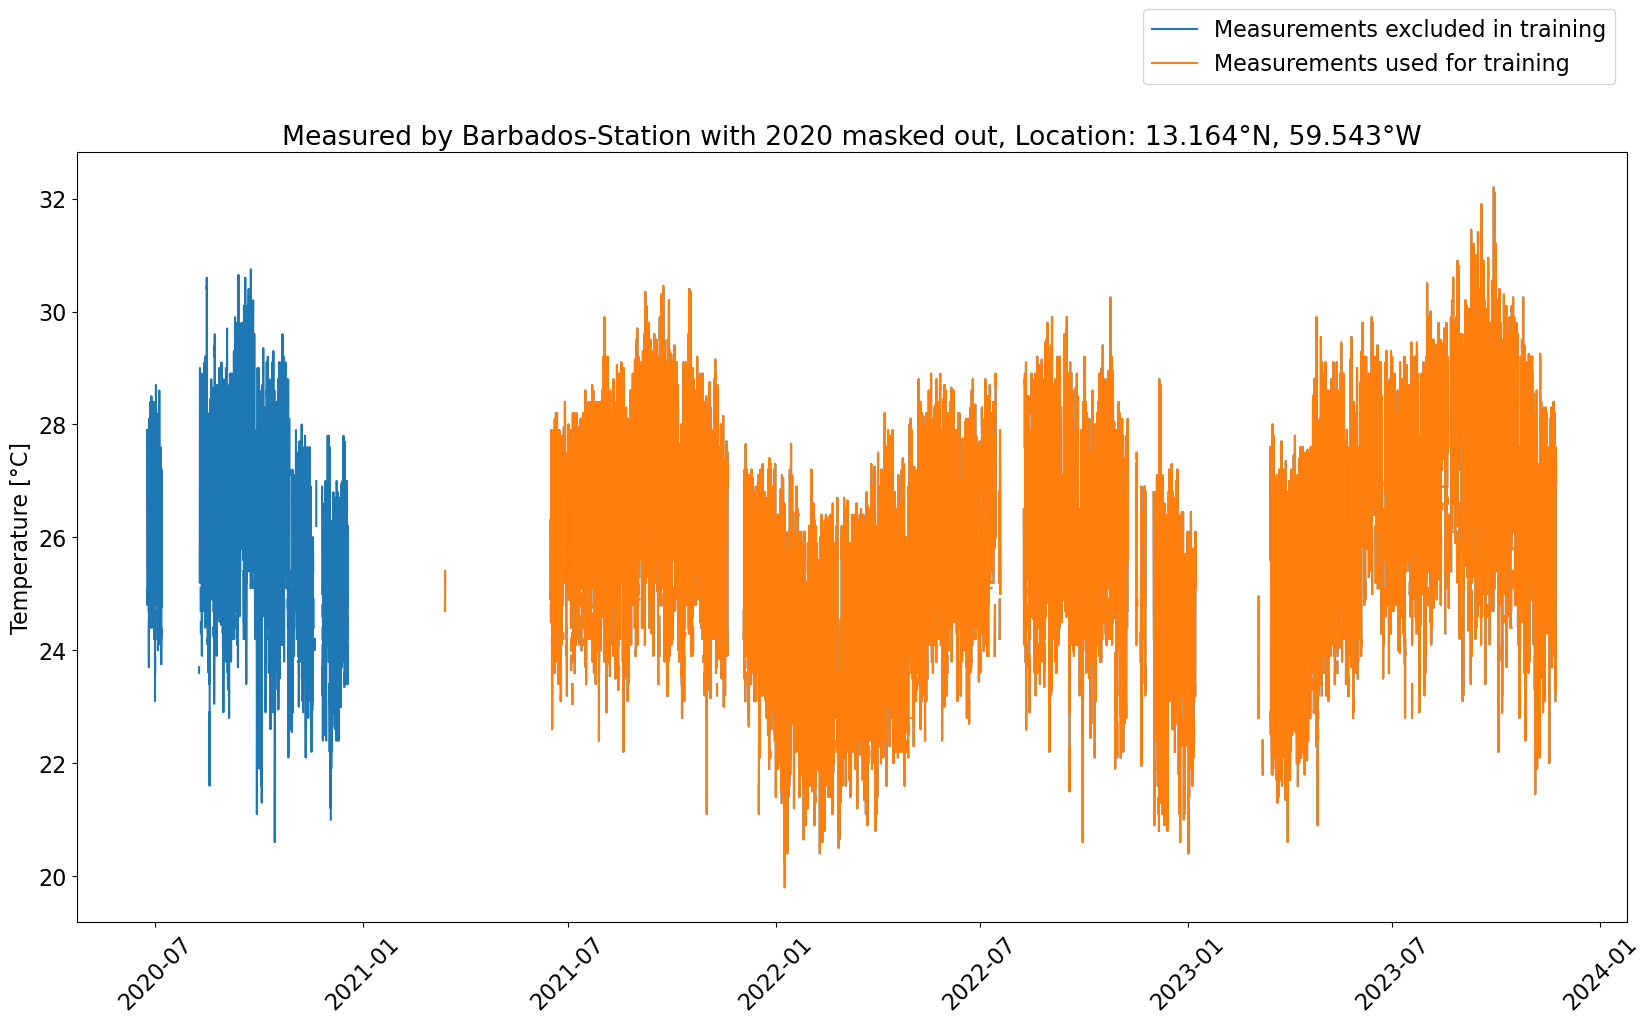
\includegraphics[width=\textwidth]{resources/images/charts/barbados_available_measurements.png}
\caption{Station in Barbados, Caribbean}
\label{fig: available_measurements_barbados}
\end{subfigure}
\caption{Available data from 3D printed Weather stations}
\label{fig: weather_stations}
\end{figure}

\begin{wrapfigure}[15]{r}{0.40\textwidth}
\centering
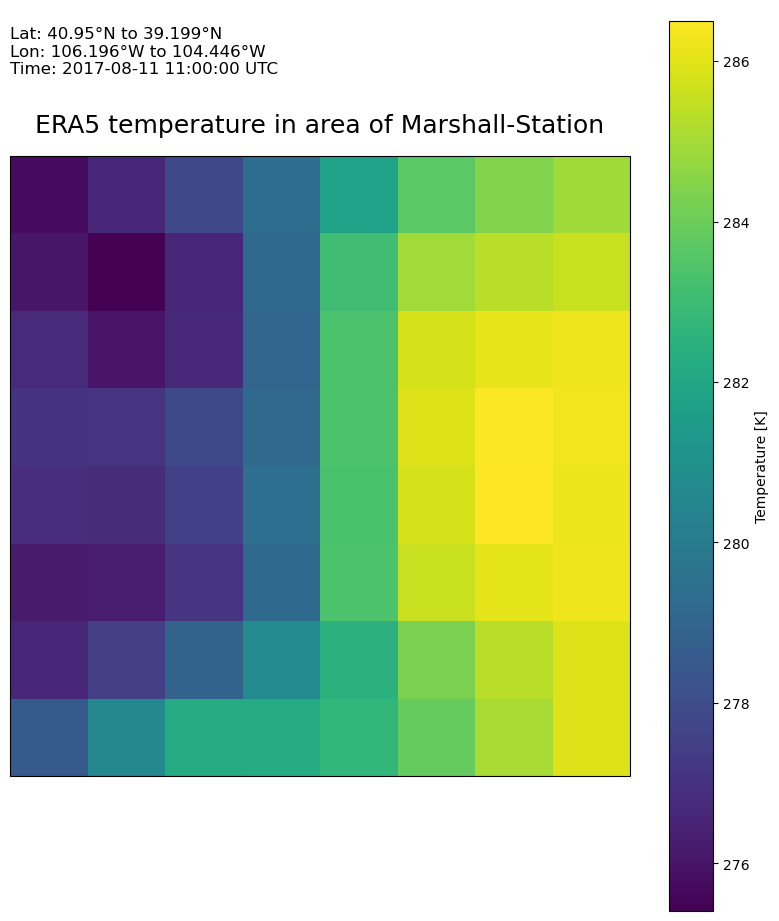
\includegraphics[width=0.38\textwidth]{resources/images/Marshall_era5.png}
\caption{ERA5 Area of the station in Marshall, Colorado}
\label{fig: era5_marshall}
\end{wrapfigure}

The station in Marshall is located between Boulder and Denver, next to Marshall Lake, at an elevation of 1,743 meters. It is less than 10 km east of South Boulder Peak, which exceeds 2,600 meters in elevation \cite{southboulderpeak}.
Further, the station is situated only about 30 km east of the Colorado Front Range, where the Rocky Mountains range in altitude between 3,250 and 4,000 meters \cite{Williams1996}.
This topographical context is visible in the ERA5 data (\autoref{fig: era5_marshall}).

Vienna lies to the west within the Vienna Basin, at a relatively low altitude just beyond the Alpine region. The Alps, which rise moderately to the west of Vienna, reach heights of up to 2,000 meters above sea level within approximately 100 km.
The ERA5 resolution is sufficient to differentiate atmospheric conditions and topographical features in this region.
The station itself resides in the north of the city on university grounds at an altitude of 159 meters.
East of it is the urban Danube Canal, separated from the station by only a main road and a railway line.

The station in Barbados stands in the parish of St. George at an altitude of 274 meters. The island is relatively flat, with its highest point being Mount Hillaby at 340 meters.
The island's size, approximately 34 km long and 23 km wide, is similar to the size of an ERA5 grid cell.
As observed in \autoref{fig: barbados}, surrounding grid cells are predominantly oceanic.
This means the ERA5 data cannot accurately capture the diurnal cycle of the station, which is influenced by its land location, while surrounding cells are mostly oceanic.

\subsection{Data Availability}

The measurements span up to late 2023, with the quantity of available temperature data varying significantly between stations. The station in Marshall, one of the oldest in the 3D-Paws project, has the most available measurements among the three stations. The weather station in Vienna has data dating back to 2017, but it has been almost entirely offline since mid-2019. The weather station in Barbados began recording in mid-2020.

\autoref{fig: weather_stations} shows the measurements from the three stations after data cleansing and conversion to an hourly basis. The measurements were provided by the US National Center for Atmospheric Research (NCAR), with most invalid values already marked. However, especially in Barbados, the sensors had more noise and occasional invalid measurements, requiring extra cleansing. Temperatures near zero and below were excluded. The conversion from minute to hourly data was done by averaging all minute values in each hour, provided there were more than 20 values available and they were not all the same. It was observed that the sensors sometimes got stuck, delivering the same value for extended periods.

The dataset for the Marshall station spans from 2017 to 2023, comprising 41,883 data points. These measurements reveal three significant data gaps, with larger intervals without data occurring in the midsummer period of 2018, late 2019 to early 2020, and the most extensive gap from September 2019 to January 2020.

For the Vienna station, measurements are available for only 12,477 hours, less than a third compared to Marshall. This is primarily due to extended downtimes starting from mid-2018, with few to no measurements except for a brief period from late 2018 to July 2019. After that, there were only sporadic data collection instances, before the station went offline in April 2022.

The Barbados station had two significant downtimes longer than a month, the largest being the first half of 2021 and the second being the first quarter of 2023. In total, the station has 17,315 hours of measurements, still less than half of the Marshall station.

\subsubsection*{Splitting into Training and Validation Data}

As explained in \autoref{sec: design}, the measurements are split into a training and validation dataset. The training dataset is used to train the model, while the validation dataset will be kept aside to compare it to what the model predicts after the training to validate if and to which extent the model learned to reconstruct the missing data. If the validation data would be included in the training data, the model would be able to predict the values it has already seen, but it would be impossible to tell if the model learned to generalize the local weather patterns.
Starting with the Marshall station, the data was sufficient to extract an entire year as validation data. Excluding a consecutive year from the training data not only allows for a comprehensive analysis of a full yearly cycle but also ensures that the model relies solely on the general weather patterns it learned from the training data to predict the values of the validation data. This approach prevents the model from potentially "cheating" by accessing information from nearby training data points, which could compromise the integrity of the validation process. It is a common practice in the machine learning field to validate data as a contiguous set, as it helps to maintain the independence and integrity of the validation process. 2021 highlighted in blue in \ref{fig: available_measurements_marshall} was the most complete year in the Marshall dataset thus it was chosen as the validation data. With the mask of 2021 applied the training data for Marshall consists of 34,188 hours of measurements which is about 82\% of the total data.

For the Vienna station, the data was split into training and validation data based on the availability of the data. The training data consists of all available data up to 2019, while the validation data is the year 2019. Resulting in 9,593 hours of measurements used as training data, which is about 77\% of the total data. The limited availability of measurements didn't allow for a full year of validation data.

The Barbados station also only had 2022 and 2023 as a complete available years, so that the decision to use the available data of 2020 as a training was a result of the lack of data as well. With the mask applied, the training data consists of 14,576 hours of measurements, which is about 84\% of the total data.


% Marshall 41883, 34188 without 2021 -> gives a ratio for validation data of 0.18

% Barbados 17315, 14576 without 2020 -> gives a ratio for validation data of 0.16

% Vienna 12477, 9593 without 2019 -> gives a ratio for validation data of 0.23

%Table with the data availability and the split into training and validation data

\begin{table}
\centering
\begin{tabular}{|c|c|c|c|c|}
\hline
Station & Total Data & Training Data & Validation Data & Validation Ratio \\
\hline
Marshall & 41,883 & 34,188 & 7,695 & 0.18 \\
Barbados & 17,315 & 14,576 & 2,739 & 0.16 \\
Vienna & 12,477 & 9,593 & 2,884 & 0.23 \\
\hline
\end{tabular}
\caption{Data availability and split into training and validation data}
\label{tab:data_split}
\end{table}

\subsubsection*{Execution of Training}

For the training and validation data, the corresponding temperature data of the 64 ERA5 grid cells in the regions of each station was obtained.
The 8x8 grid cells were chosen to be centered as well as possible around each weather station, given the specific ERA5 coordinates.
The ERA5 data was also preprocessed using the code pipeline described in \autoref{sec: implementation}.
Then, the CNN with the architecture described in \autoref{subsec:cnn} was trained on the training data. The training was done in batches of 4 data points, which are, in hour case, the hourly steps at a time. The model was trained for up to 300,000 iterations, which, therefore, depend on the dataset size between 8 and 31 epochs. The training was done on the Supercomputer "Levante" of the German Climate Computing Center, which made it possible to complete training runs in just a few hours. However, the training can be done in the same way on almost any machine. During the training, in the scientific process, where the approach is un-proven to work, it is especially important to validate multiple times during the training to calculate not only the loss function over the model for the training data, but over the validation data. This is done to prevent overfitting, a so-called phenomenon where the model in the aim to minimize the loss for the training data, which is what training using backpropagation is exactly at it is core, starts to learn the noise and any potential specifics of the training data so well, that it loses it is ability to generalize and the loss for the validation data starts to increase. This is a sign that the model is overfitting and the training should be stopped. The model that is then chosen is the one that performed best on the validation data. To allow for that, not only was the ERA5 data for the training data provided to the machine learning architecture but the validation ERA5 data was also paired with the expected output for these, the masked measurements of the weather station.

Training runs have been completed for all stations with up to 1 million iterations, but the best models were in most cases, already found between 300 and 500 thousand iterations. The models were then applied to the ERA5 data at all the hours in the validation data set of each station, to analyze the performance of the model for each station. 

\subsection{Validation Methods}

\begin{figure}
    \centering
    \begin{subfigure}{0.35\textwidth}
        \centering
        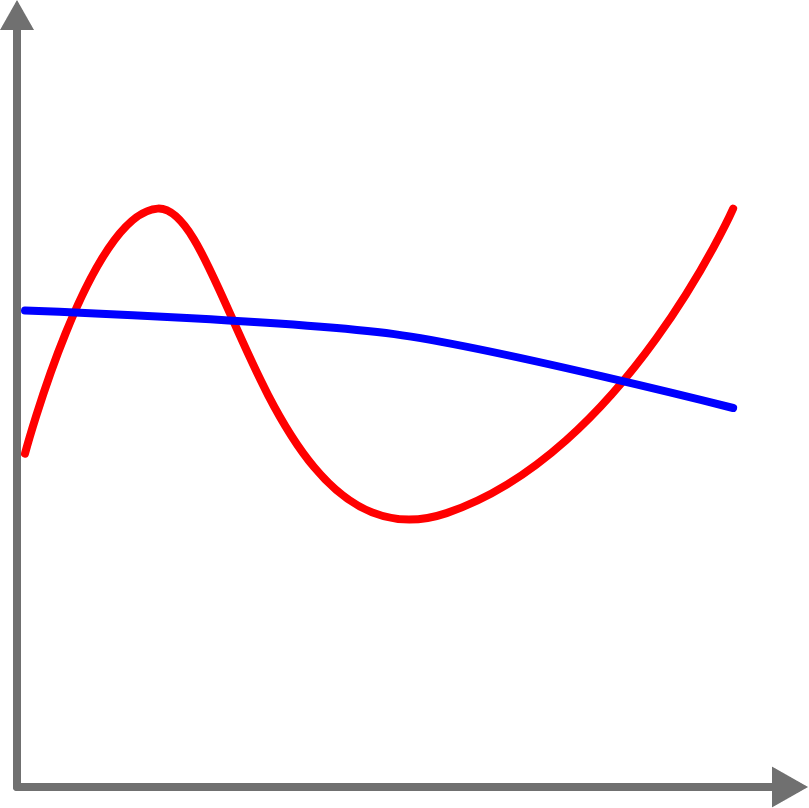
\includegraphics[width=0.7\textwidth]{resources/images/low_rmse.png}
        \caption{Low RMSE, low Correlation Coefficient}
        \label{fig: low_rmse}
    \end{subfigure}
    \hspace{0.5cm}
    \begin{subfigure}{0.35\textwidth}
        \centering
        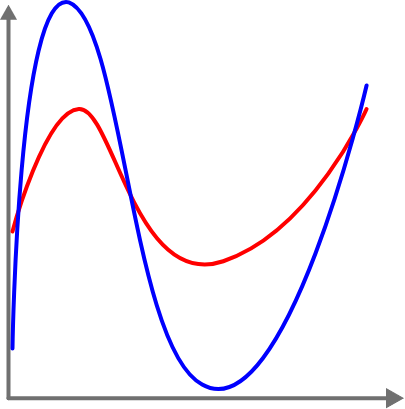
\includegraphics[width=0.7\textwidth]{resources/images/high_corr.png}
        \caption{High Correlation Coefficient, high RMSE}
        \label{fig: high_corr}
    \end{subfigure}
    \caption{Comparison of the RMSE and Correlation Coefficient}
\end{figure}

As numerical measures of quality, the Root Mean Squared Error (RMSE) and the correlation coefficient were calculated. The RMSE is a measure of the differences between predicted and observed values, while the correlation coefficient quantifies the strength and direction of the linear relationship between the two datasets. 


\subsubsection*{Root Mean Squared Error (RMSE)}

To quantify how far apart the reconstructed temperature series $\hat{y}$ is from the measured temperature series $y$, where both series have $n$ different timesteps and thus can be seen as vectors, most commonly the root mean squared error (RMSE) comes to help, which is strongly connected to the Euclidean norm of the difference between both vectors $\hat{y} - y$. However, a simple mean absolute error (MAE), also called the Manhattan norm, could seem most intuitive and easiest to understand. It would be calculated just by adding all absolute differences up before dividing it by the length of the series. The RMSE is favored in machine learning and statistics because it penalizes larger differences more than smaller ones, which is more in line with the human perception of errors. 

\begin{equation}
    \text{RMSE} = \sqrt{\frac{1}{n} \sum_{i=1}^{n} (y_i - \hat{y}_i)^2}
    \label{eq:rmse}
\end{equation}

\begin{equation}
    \text{MAE} = \frac{1}{n} \sum_{i=1}^{n} |y_i - \hat{y}_i|
    \label{eq:mae}
\end{equation}

When converting \autoref*{eq:rmse}, it can be seen how the RMSE is connected to the Euclidean norm:

\begin{equation}
  \text{RMSE} \cdot \sqrt{n} = \sqrt{\sum_{i=1}^{n} (y_i - \hat{y}_i)^2} = \| y - \hat{y} \|_2  
  \label{eq:rmse_euclid}
\end{equation}

The Euclidean norm $\| y - \hat{y} \|_2$, of a coordinate in our case the error $\hat{y} - y$ can be imagined as the diagonal distance between the origin and the point with these coordinates. For demonstration purposes, a right triangle in 2-dimensional space can be imagined with the errors at 2 validation timesteps as the legs. The RMSE over both errors would be proportional to the hypothenuse of that triangle which is more dependent on the length of the longer leg than the shorter one. The Manhattan norm (\autoref{eq:mae}), on the other hand, which received its name from the gridded street system of Manhattan is not based on the diagonal distance, but the distance a taxicab in Manhattan would have to drive to travel along the hypothenuse, the equally weighted sum of the legs.

\subsubsection*{Pearson Correlation Coefficient}

The Pearson correlation coefficient (in the following called correlation coefficient), is a measure of the strength and direction of a linear relationship between two variables. It ranges from -1 to 1, where 1 indicates a perfect positive linear relationship, -1 is a perfect negative linear relationship, and 0 is no linear relationship. The correlation coefficient is calculated as follows:

\begin{equation}
    \text{Correlation Coefficient} = \frac{\sum_{i=1}^{n} (y_i - \bar{y})(\hat{y}_i - \bar{\hat{y}})}{\sqrt{\sum_{i=1}^{n} (y_i - \bar{y})^2 \sum_{i=1}^{n} (\hat{y}_i - \bar{\hat{y}})^2}}
    \label{eq:correlation}
\end{equation}
    
Where $\bar{y}$ and $\bar{\hat{y}}$ are the mean values of the measured and the model output temperature series, respectively. The correlation coefficient is a measure of how well the model output follows the general trend of the measured data. \cite{Zou2003Correlation}

\subsection{Validation of the Models}

\subsubsection*{Marshall-Station}

\begin{figure}
    \centering
    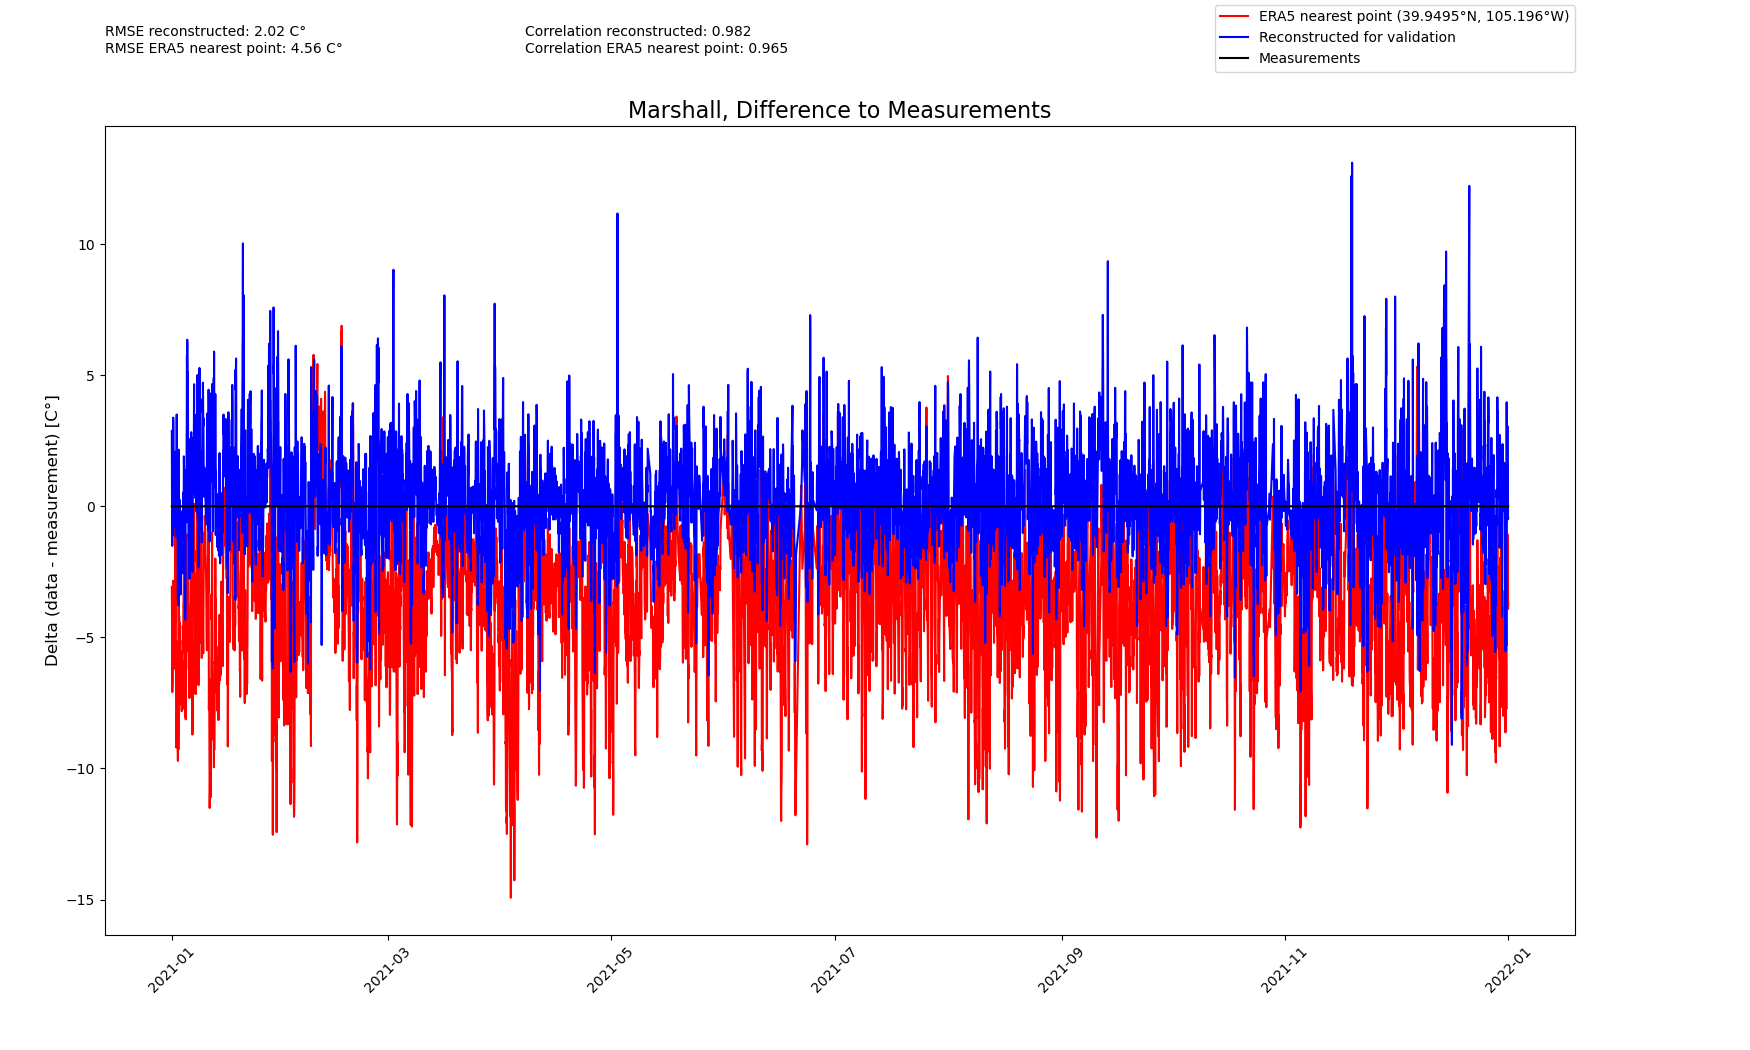
\includegraphics[width=1.07\textwidth]{resources/images/charts/marshall_eval_grib_final/Marshall, Difference to Measurements.png}
    \caption{Difference between reconstructed and measured temperature for Marshall-Station}
    \label{fig: marshall_diff}
\end{figure}

To begin with Marshall the occasion with the most available training data, all by the model predicted temperatures for the hourly measurements of the validation dataset have been plotted in \autoref{fig: marshall_diff} with a blue line against the ground truth in black. Given the high number of hourly timesteps along the x-axis spanning the year 2021, for the sake of readability, the temperature differentials are plotted on the y-axis instead of the absolute temperatures. Above the chart the over the whole hourly validation data calculated RMSE and Correlation of the reconstructed series are written. The RMSE for the Marshall station is 2.02°C, which is the highest value among the three weather stations, which models have been trained for. To compare the RMSE to what a direct read out of ERA5 would have been, the plot includes in red the temperature at each timestep at the nearest ERA5 grid point, at the coordinates 39.950° N, 106.196° W. The grid point's location is exactly the location of the weather station in Marshall (see \autoref{fig: available_measurements_marshall}). But the RMSE between the measurements and the temperature time series of that ERA5 grid point, is 4.56°C, which is more than twice as high. Considering that the model was trained on the ERA5 data of the 8x8 grid cells around the station, the model was able to reduce the error significantly. The ERA5 data, as seen in the chart has a substantial low-bias compared to the station which directly relates to the fact that the grid cell of the station already reaches into the Rocky Mountains, as described above. Thus it is especially important, that the reconstruction not just has a lower RMSE which could be achieved in this case just by correcting the low-bias but also beats it is training data in terms of correlation. The calculated correlation coefficient over the validation year 2021 on an hourly basis for the reconstructed temperature and the measurements is 0.982 compared to 0.965 for the ERA5 nearest grid point a significant improvement.

\begin{figure}
    \centering
    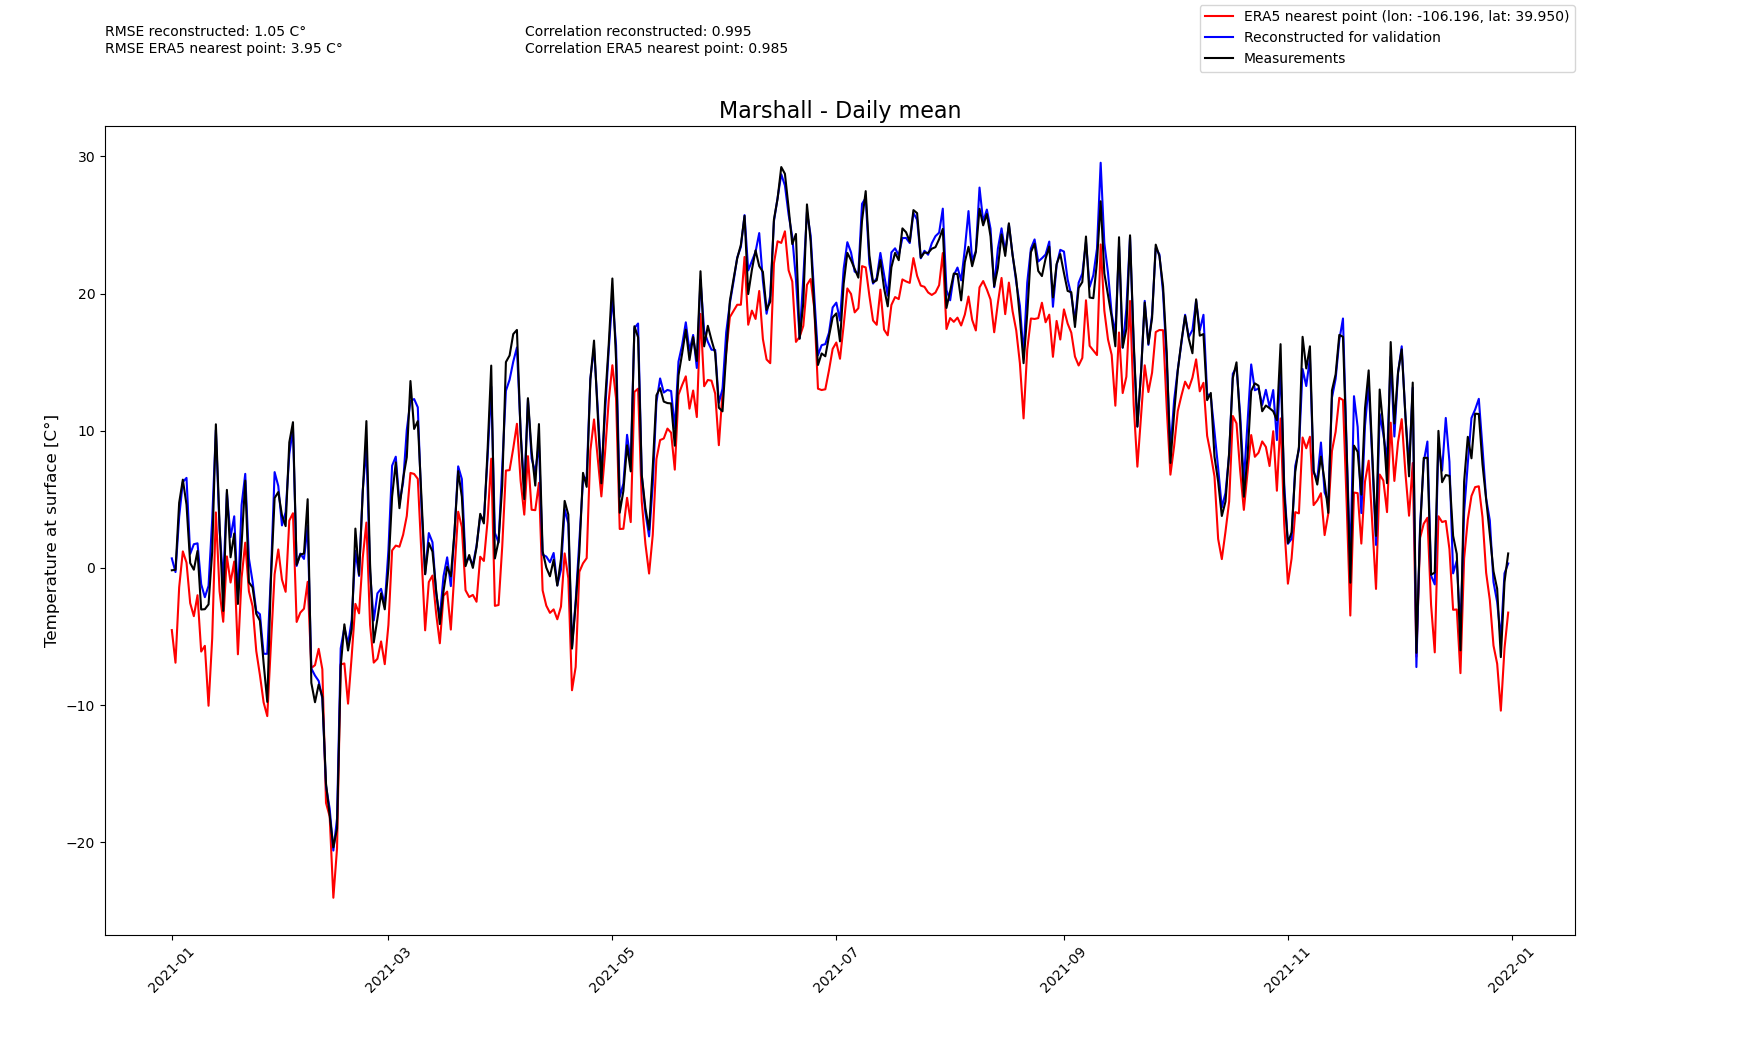
\includegraphics[width=1.07\textwidth]{resources/images/charts/marshall_eval_grib_final/Marshall - Daily mean.png}
    \caption{Reconstructed temperature vs measured temperature for Marshall-Station (Daily mean)}
    \label{fig: marshall_daily}
\end{figure}

Even better is the performance of the model when the hourly values are combined again with daily means, as in \autoref{fig: marshall_daily}. The chart shows the daily mean temperature of the three different series, known from the previous chart over 2021. In this case, the reduced number of timesteps allows for an absolute temperature scale on the y-axis and therefore makes the performance of the model visually appealing as well, the RMSE on a daily basis for the prediction is almost halved the original one at 1.05°C, while the correlation coefficient is even higher as well at 0.995, the ERA5 correlation coefficient improved significantly as well, however, the RMSE didn't as the ERA5 data is impacted drastically by the low-bias.

\begin{figure}
    \centering
    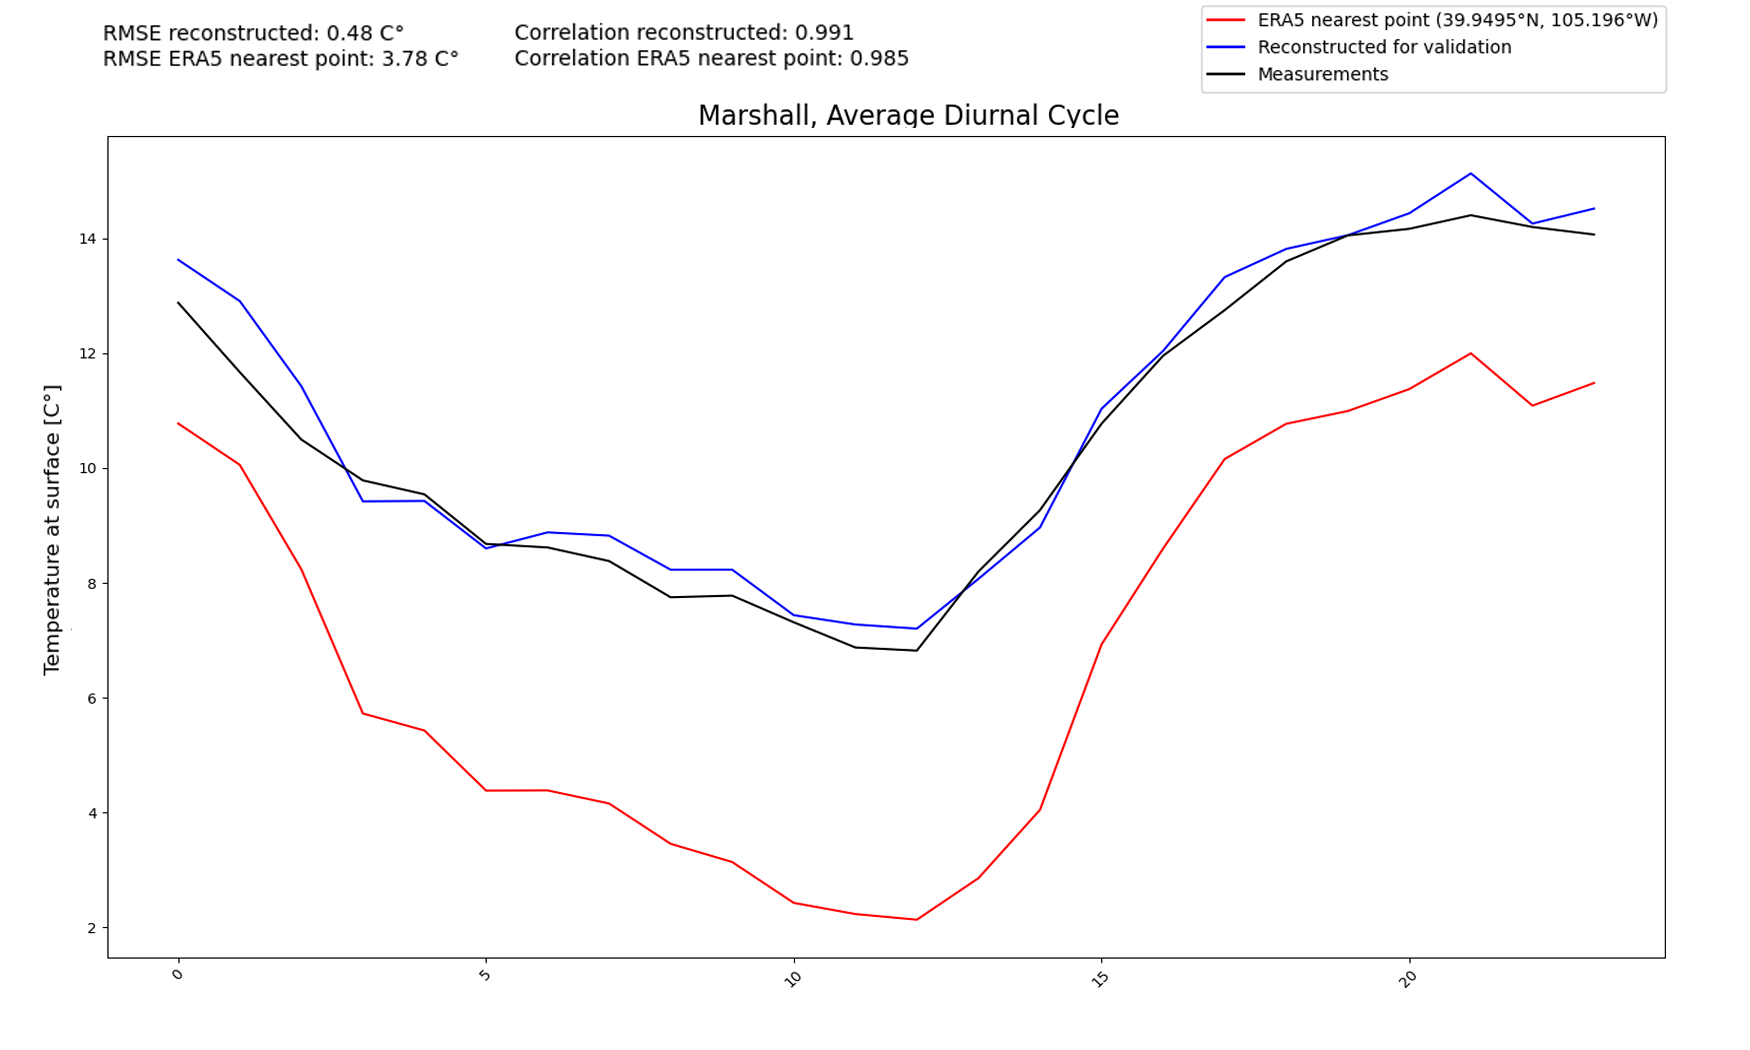
\includegraphics[width=1.07\textwidth]{resources/images/charts/marshall_eval_grib_final/Marshall, Average Diurnal Cycle.png}
    \caption{Reconstructed temperature vs measured temperature for Marshall-Station (Average Diurnal Cycle)}
    \label{fig: marshall_diurnal}
\end{figure}

\autoref{fig: marshall_diurnal} makes clear, that the improvement in RMSE and correlation coefficient of the daily analysis was not caused by potential issues in the model to predict the diurnal cycle correctly but by noise reduction in general. In \autoref{fig: marshall_diurnal} the average diurnal cycle of the reconstructed temperature is plotted against the measured temperature and the temperature series of ERA5. This means that over all the days in 2021, for each of the 24 hours, an average temperature was calculated and plotted for the three series. As all measurements, have been recorded in universal time code (UTC), which is also the time in ERA5, the x-axis is also using UTC, which is apart from the daylight savings time 6 hours ahead of Colorado. It can be observed that ERA5 has a higher amplitude in the diurnal cycle than the weather station and that the model is capable of correcting that.

It is not surprising, that the RMSE and correlation coefficient improve the more the data is aggregated, so it is also important to look at the hourly values again and go into detail. To allow the details to appear on a plot, the x-axis can be cropped to a shorter period, as in \autoref{fig: marshall_7day}, where the x-axis includes 168 hours, equivalent to 7 days. The chart is chosen to be representative, while some weeks have a better fitting than others. In this case, it can be seen, that even in the measurements of 2021, minor gaps happened. For example  


\begin{figure}
    \centering
    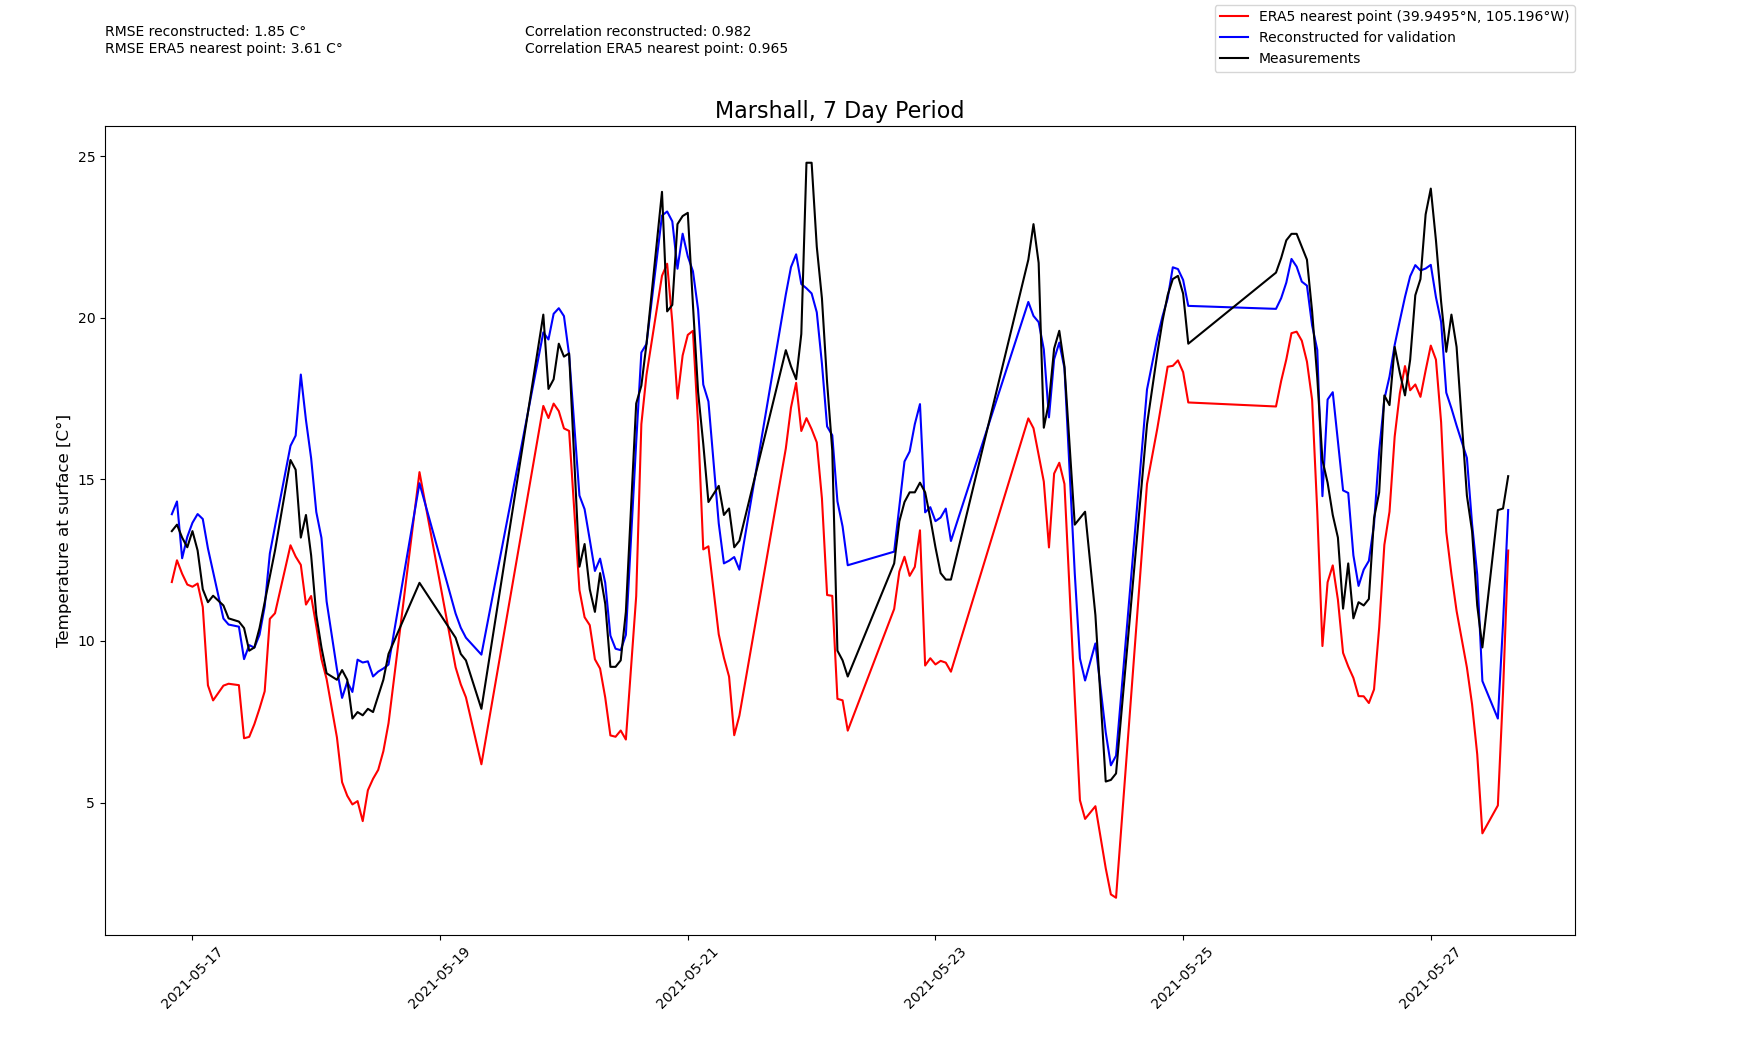
\includegraphics[width=1.07\textwidth]{resources/images/charts/marshall_eval_grib_final/Marshall, 7 Day Period_1_2_3.png}
    \caption{Reconstructed temperature vs measured temperature for Marshall-Station (7 Day Period)}
    \label{fig: marshall_7day}
\end{figure}

\begin{figure}
    \centering
    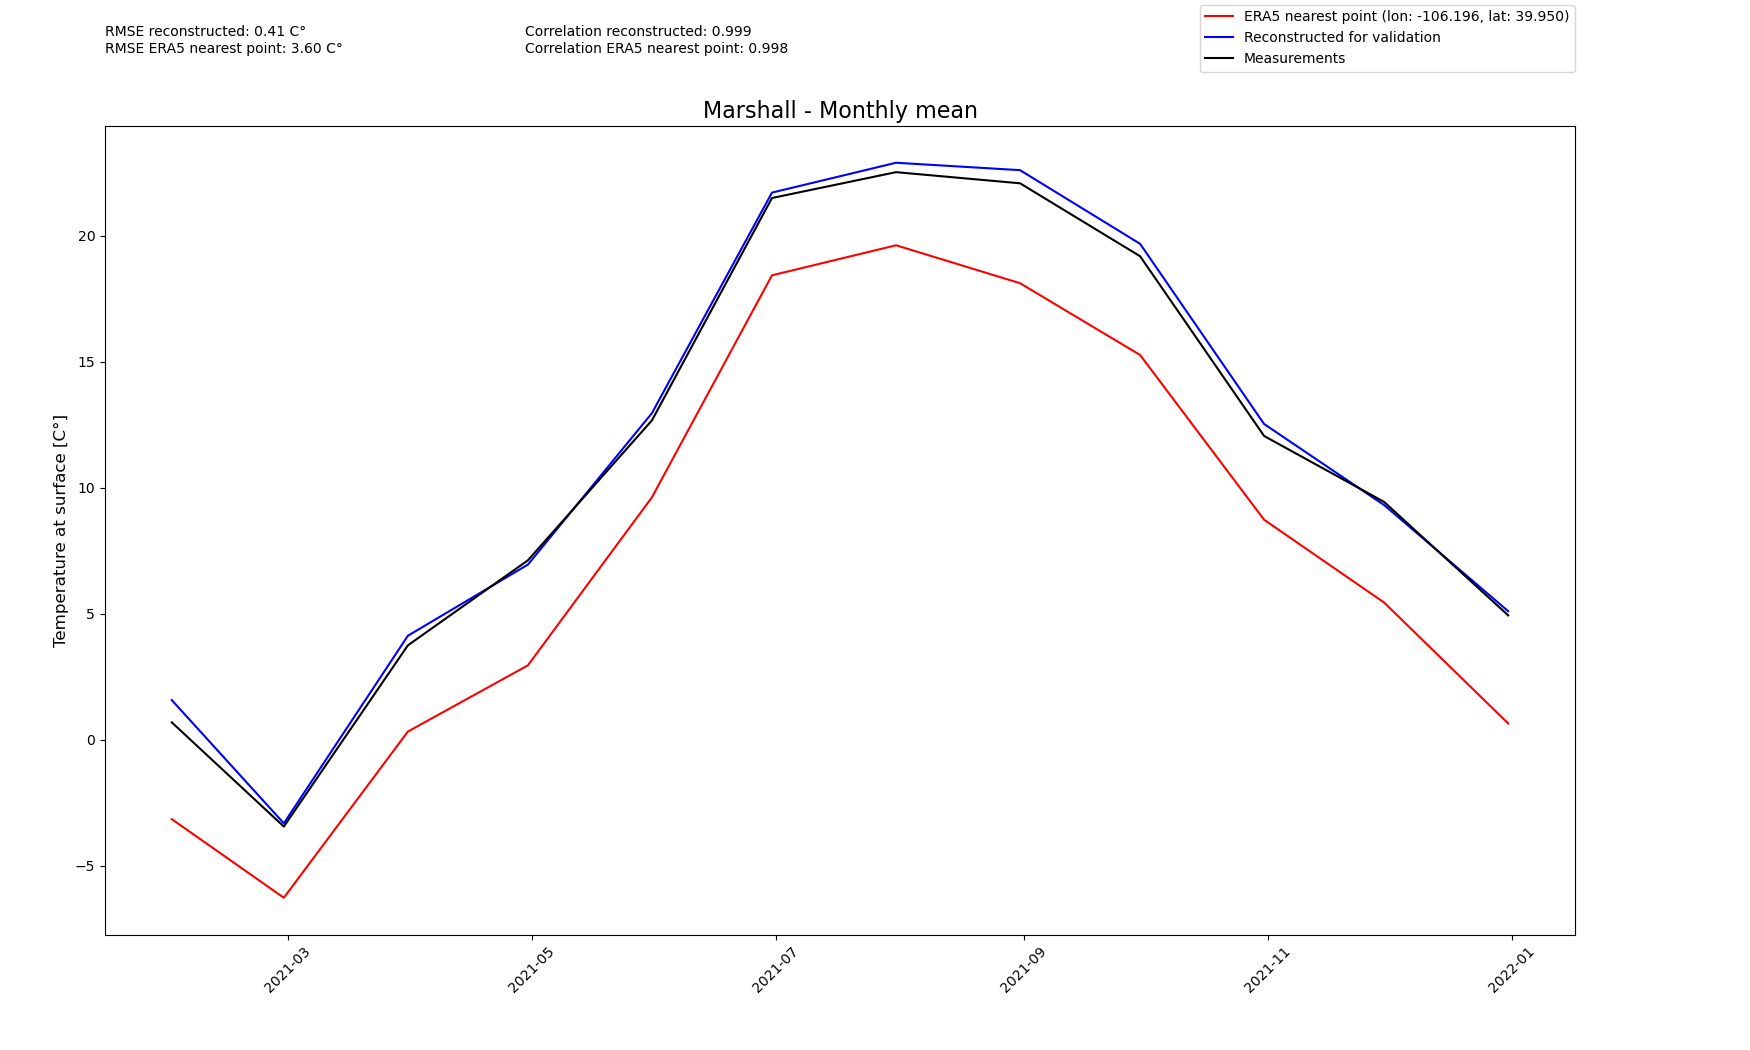
\includegraphics[width=1.07\textwidth]{resources/images/charts/marshall_eval_grib_final/Marshall - Monthly mean.png}
    \caption{Reconstructed temperature vs measured temperature for Marshall-Station (Monthly mean)}
\end{figure}


\subsubsection*{Vienna-Station}

\begin{figure}
    \centering
    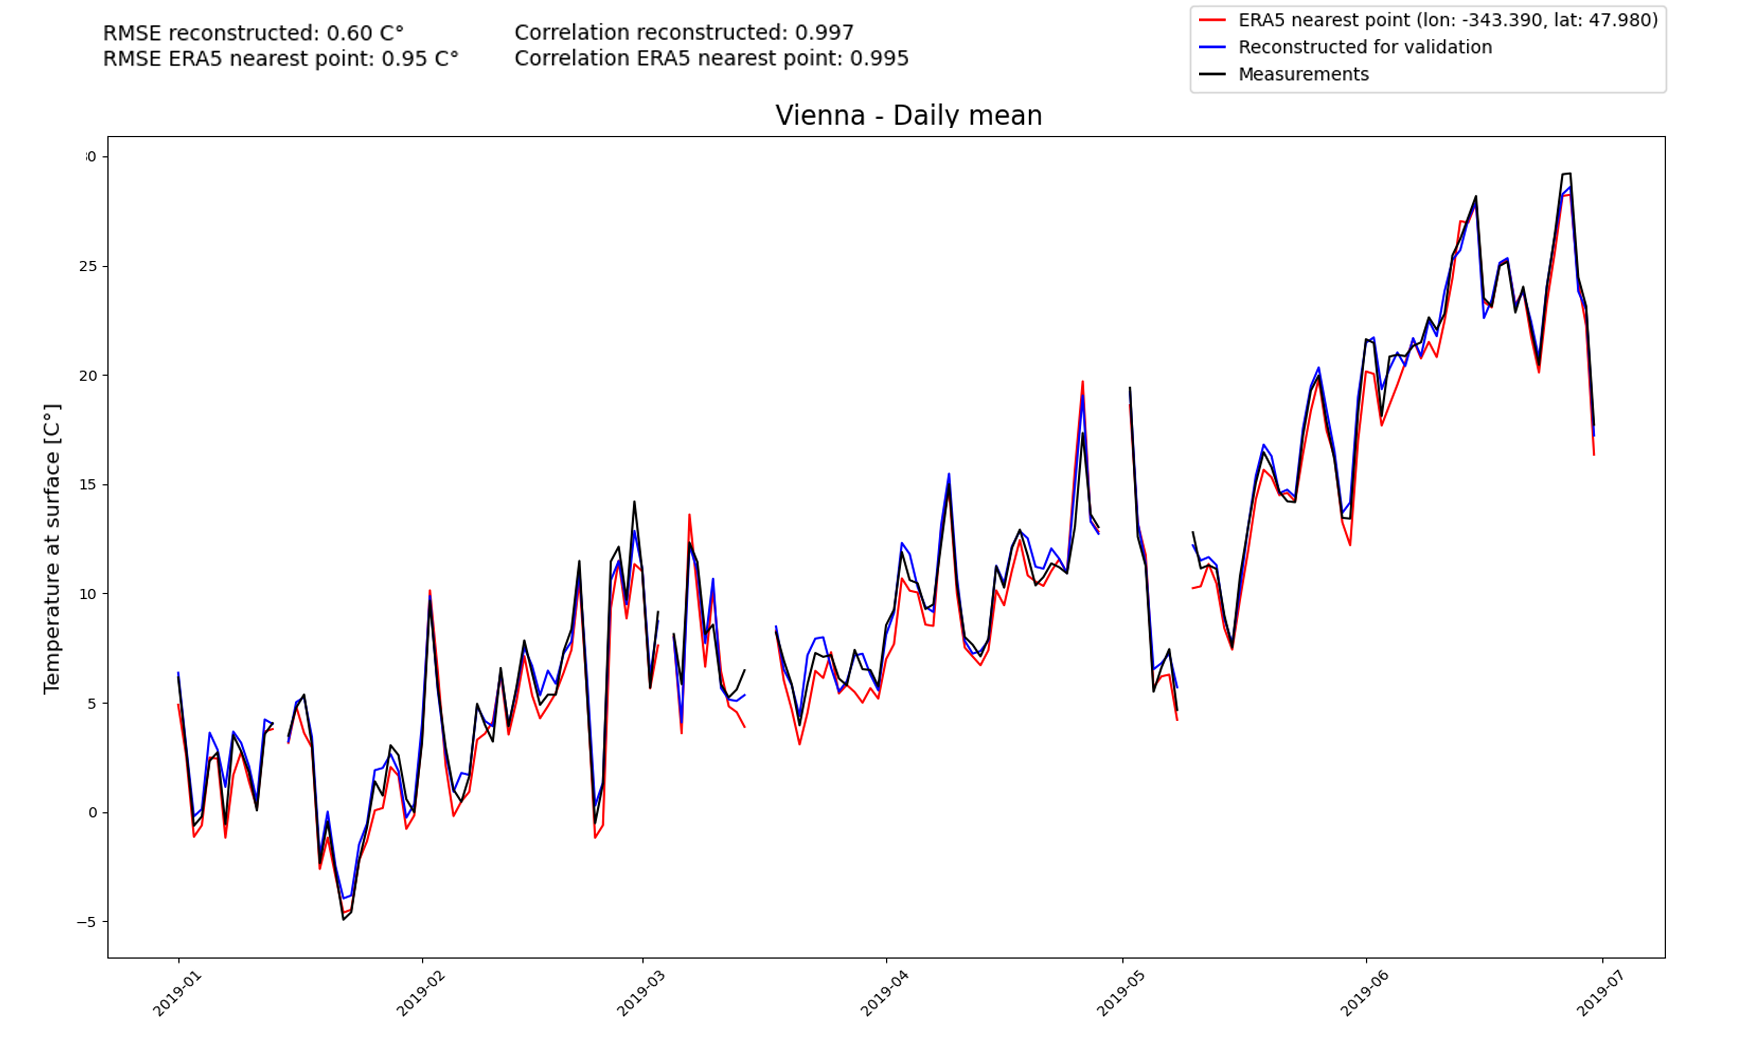
\includegraphics[width=1.07\textwidth]{resources/images/charts/vienna_eval_grib_final/Vienna - Daily mean.png}
    \caption{Reconstructed temperature for Vienna-Station (Daily mean)}
\end{figure}

\begin{figure}
    \centering
    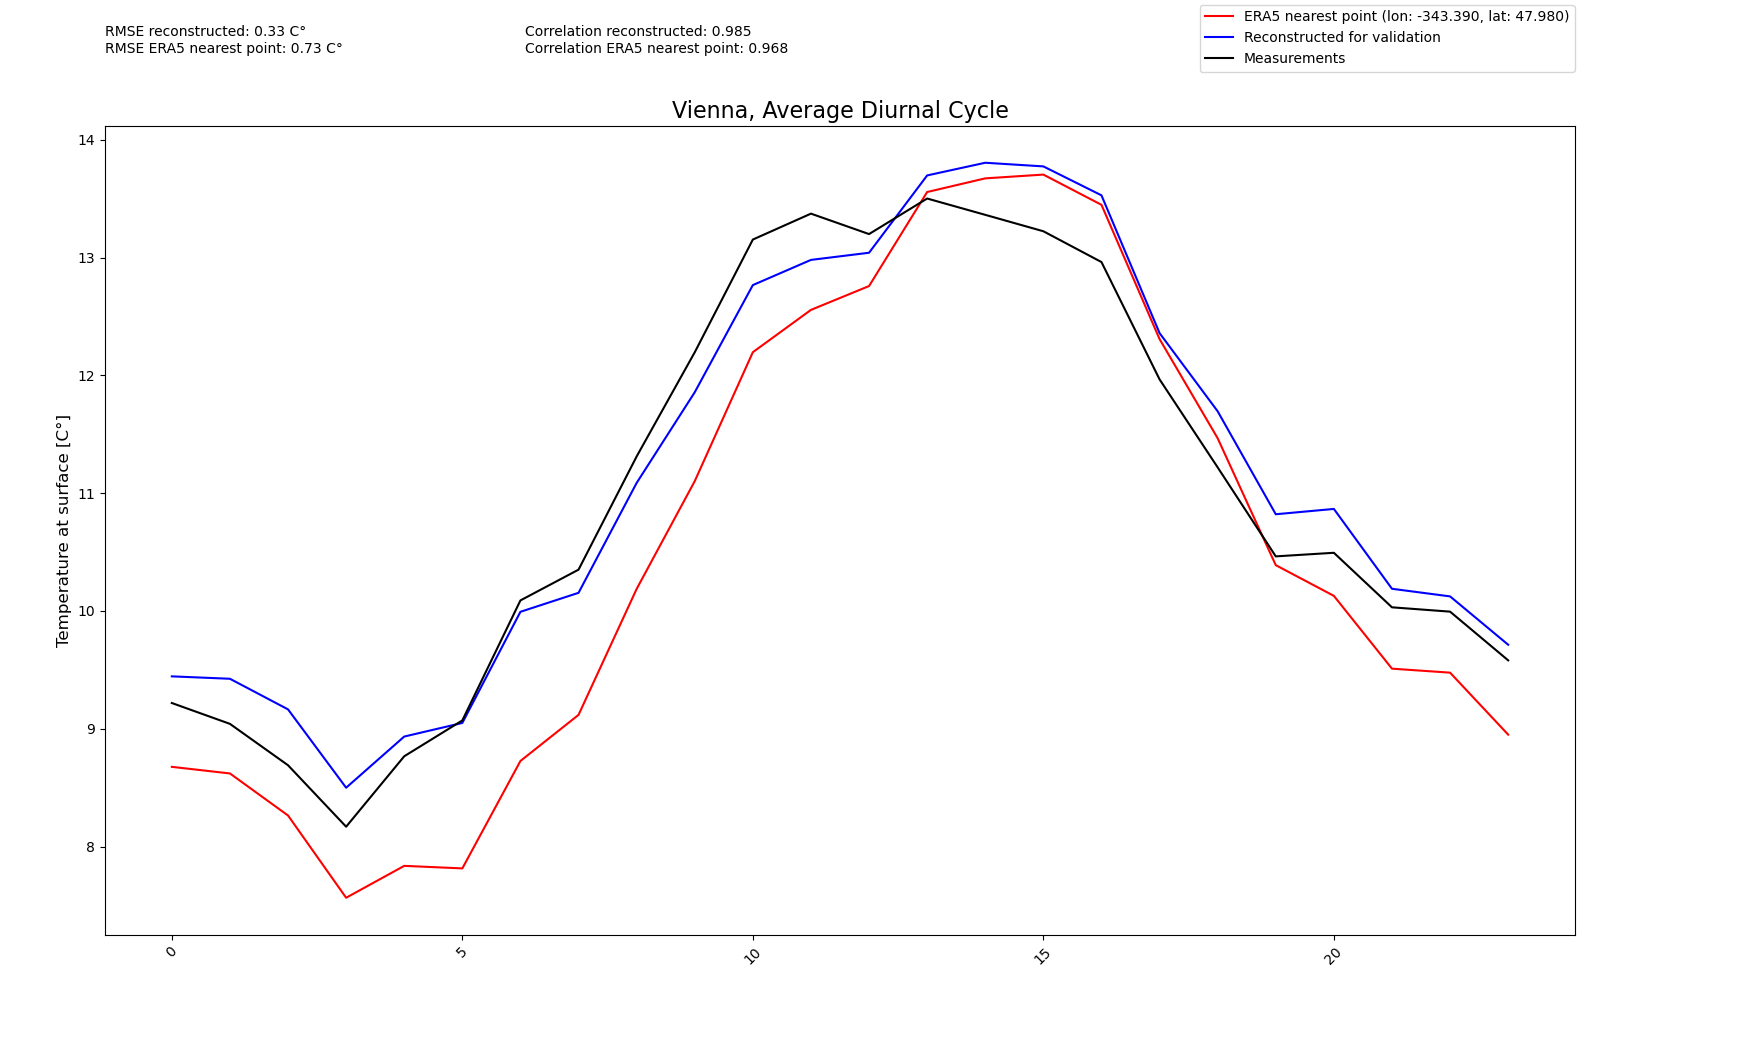
\includegraphics[width=1.07\textwidth]{resources/images/charts/vienna_eval_grib_final/Vienna, Average Diurnal Cycle.png}
    \caption{Measured temperature for Vienna-Station (Average Diurnal Cycle)}
\end{figure}

\newpage

\subsubsection*{Barbados-Station}

\begin{figure}
    \centering
    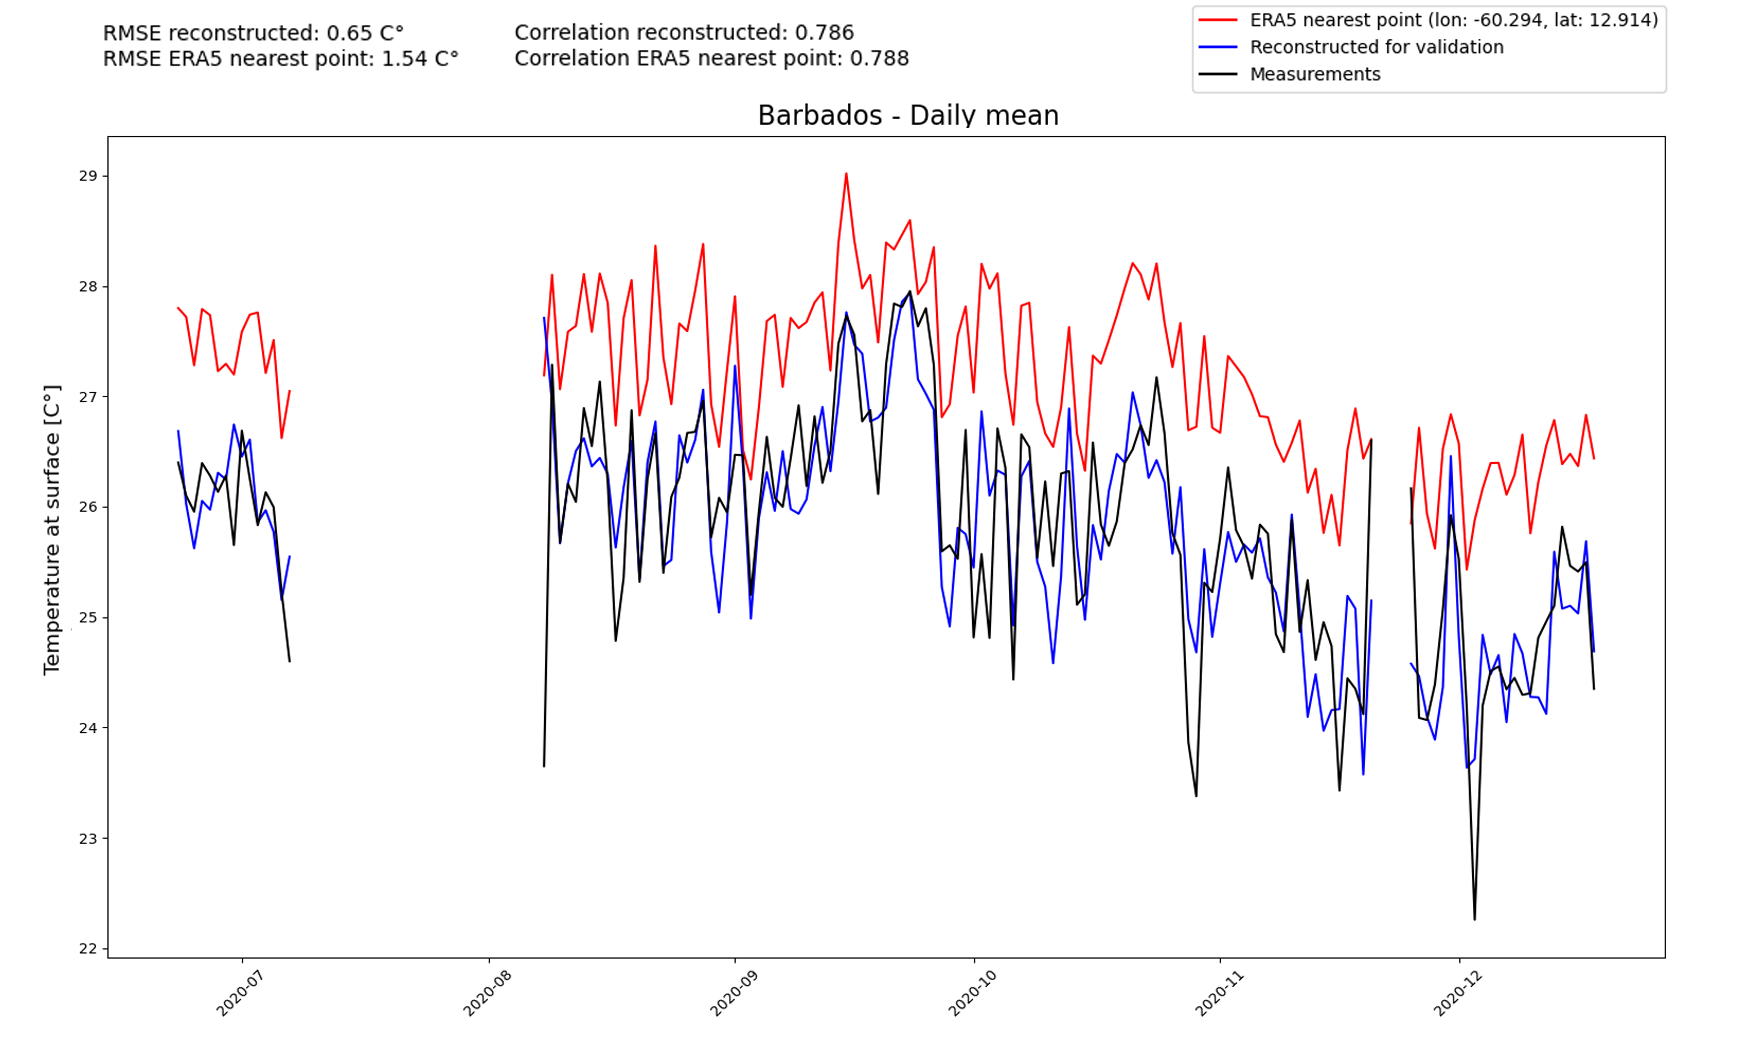
\includegraphics[width=1.07\textwidth]{resources/images/charts/barbados_eval_grib_final/Barbados - Daily mean.png}
    \caption{Reconstructed temperature for Barbados-Station (Daily mean)}
\end{figure}

\begin{figure}
    \centering
    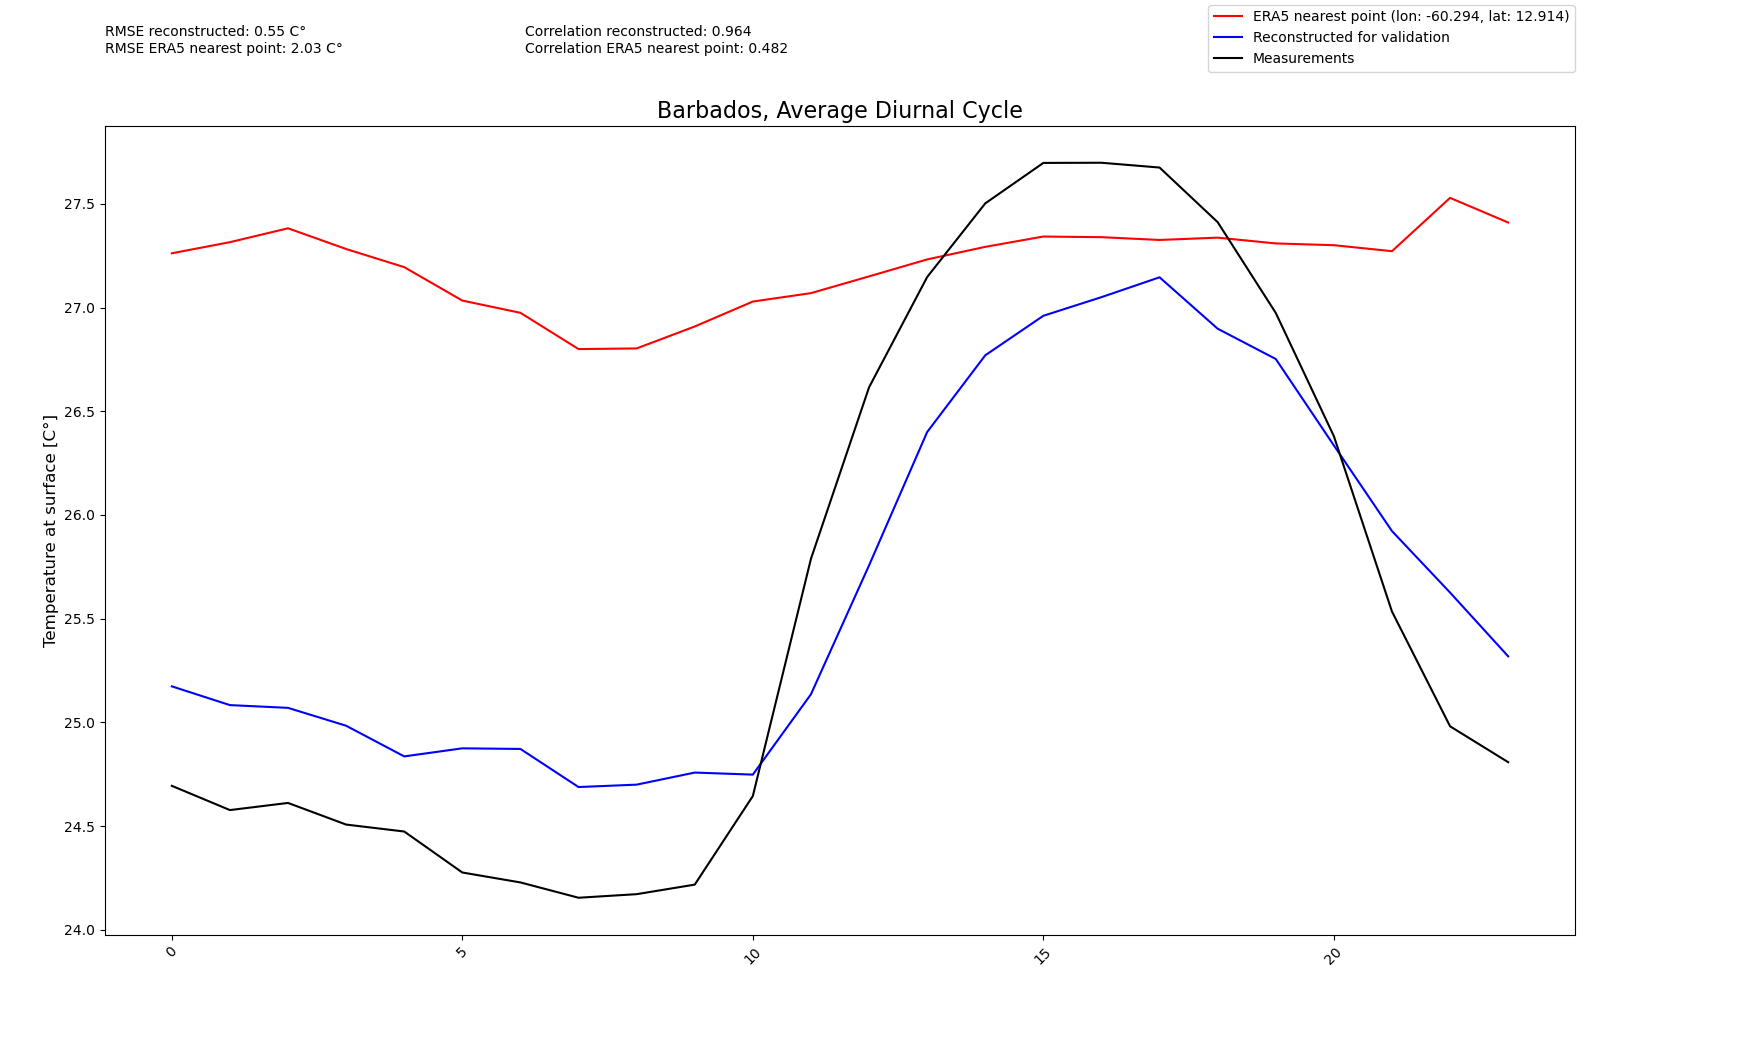
\includegraphics[width=1.07\textwidth]{resources/images/charts/barbados_eval_grib_final/Barbados, Average Diurnal Cycle.png}
    \caption{Measured temperature for Barbados-Station (Average Diurnal Cycle)}
\end{figure}

\newpage